% This document, similar to Estimation.Rnw, takes into account the remarks of advisors given during the meeting of the 6th of December 2021.

\documentclass[a4paper,oneside,12pt,titlepage]{article}\usepackage[]{graphicx}\usepackage[]{color}
% maxwidth is the original width if it is less than linewidth
% otherwise use linewidth (to make sure the graphics do not exceed the margin)
\makeatletter
\def\maxwidth{ %
  \ifdim\Gin@nat@width>\linewidth
    \linewidth
  \else
    \Gin@nat@width
  \fi
}
\makeatother

\definecolor{fgcolor}{rgb}{0.345, 0.345, 0.345}
\newcommand{\hlnum}[1]{\textcolor[rgb]{0.686,0.059,0.569}{#1}}%
\newcommand{\hlstr}[1]{\textcolor[rgb]{0.192,0.494,0.8}{#1}}%
\newcommand{\hlcom}[1]{\textcolor[rgb]{0.678,0.584,0.686}{\textit{#1}}}%
\newcommand{\hlopt}[1]{\textcolor[rgb]{0,0,0}{#1}}%
\newcommand{\hlstd}[1]{\textcolor[rgb]{0.345,0.345,0.345}{#1}}%
\newcommand{\hlkwa}[1]{\textcolor[rgb]{0.161,0.373,0.58}{\textbf{#1}}}%
\newcommand{\hlkwb}[1]{\textcolor[rgb]{0.69,0.353,0.396}{#1}}%
\newcommand{\hlkwc}[1]{\textcolor[rgb]{0.333,0.667,0.333}{#1}}%
\newcommand{\hlkwd}[1]{\textcolor[rgb]{0.737,0.353,0.396}{\textbf{#1}}}%
\let\hlipl\hlkwb

\usepackage{framed}
\makeatletter
\newenvironment{kframe}{%
 \def\at@end@of@kframe{}%
 \ifinner\ifhmode%
  \def\at@end@of@kframe{\end{minipage}}%
  \begin{minipage}{\columnwidth}%
 \fi\fi%
 \def\FrameCommand##1{\hskip\@totalleftmargin \hskip-\fboxsep
 \colorbox{shadecolor}{##1}\hskip-\fboxsep
     % There is no \\@totalrightmargin, so:
     \hskip-\linewidth \hskip-\@totalleftmargin \hskip\columnwidth}%
 \MakeFramed {\advance\hsize-\width
   \@totalleftmargin\z@ \linewidth\hsize
   \@setminipage}}%
 {\par\unskip\endMakeFramed%
 \at@end@of@kframe}
\makeatother

\definecolor{shadecolor}{rgb}{.97, .97, .97}
\definecolor{messagecolor}{rgb}{0, 0, 0}
\definecolor{warningcolor}{rgb}{1, 0, 1}
\definecolor{errorcolor}{rgb}{1, 0, 0}
\newenvironment{knitrout}{}{} % an empty environment to be redefined in TeX

\usepackage{alltt}

\usepackage{booktabs}

\usepackage[utf8]{inputenc}
\usepackage[T1]{fontenc}
\usepackage{graphicx}
\usepackage[version=4]{mhchem}
\usepackage[scientific-notation=true]{siunitx}
\usepackage{gensymb}
\usepackage[top=2.5cm, bottom=3cm, left=2.5cm, right=2.5cm]{geometry}
\usepackage{float}
\usepackage{amsmath,amsfonts,amsthm} % Math packages
\title{Preliminary Outlier Detection in Missing Values Free data}
\IfFileExists{upquote.sty}{\usepackage{upquote}}{}
\begin{document}
\maketitle
Problems : Valid estimation of a composition of rocks.
\begin{enumerate}
\item composition of major elements with outliers
\item composition of major elements with outliers and missing values
\item : composition of major elements with outliers and missing values
\item : composition of all elements with outliers and missing values
\end{enumerate}

An initial goal of this work is to provide robust estimates of the composixtion of each rock. This problem is made difficult by the presence of both missing values (laboratories did not measure any composition) and outliers (the measures reported are extreme).

Setting aside the problem of missing values for now, one may look at a subcomposition $\mathbf{x} \in \mathbb{S}^D$ of oxides of major elements.

One begin by importing a dataset, for example GeoPT48, a monzonite.





\begin{knitrout}
\definecolor{shadecolor}{rgb}{0.969, 0.969, 0.969}\color{fgcolor}\begin{kframe}
\begin{alltt}
\hlkwd{setwd}\hlstd{(}\hlstr{"/home/max/Documents/MStatistics/MA2/Thesis/Repository/"}\hlstd{)}
\hlstd{data} \hlkwb{<-} \hlkwd{read_csv}\hlstd{(}\hlstr{"data/raw/GeoPT48 -84Ra.csv"}\hlstd{)}
\end{alltt}


{\ttfamily\noindent\itshape\color{messagecolor}{\#\# \\\#\# -- Column specification --------------------------------------------------------\\\#\# cols(\\\#\# \ \ .default = col\_double(),\\\#\# \ \ Laboratory = col\_character(),\\\#\# \ \ Au = col\_logical(),\\\#\# \ \ N = col\_logical(),\\\#\# \ \ Os = col\_logical()\\\#\# )\\\#\# i Use `spec()` for the full column specifications.}}\begin{alltt}
\hlstd{data2} \hlkwb{<-} \hlkwd{read_csv}\hlstd{(}\hlstr{"data/raw/GeoPT46 -84Ra.csv"}\hlstd{)}
\end{alltt}


{\ttfamily\noindent\color{warningcolor}{\#\# Warning: Missing column names filled in: 'X1' [1]}}

{\ttfamily\noindent\itshape\color{messagecolor}{\#\# \\\#\# -- Column specification --------------------------------------------------------\\\#\# cols(\\\#\# \ \ .default = col\_double(),\\\#\# \ \ Laboratory = col\_character(),\\\#\# \ \ Ir = col\_logical(),\\\#\# \ \ N = col\_logical(),\\\#\# \ \ Os = col\_logical(),\\\#\# \ \ Rh = col\_logical(),\\\#\# \ \ Ru = col\_logical()\\\#\# )\\\#\# i Use `spec()` for the full column specifications.}}\end{kframe}
\end{knitrout}
Then, one looks at the subcomposition of major elements :
\begin{knitrout}
\definecolor{shadecolor}{rgb}{0.969, 0.969, 0.969}\color{fgcolor}\begin{kframe}
\begin{alltt}
\hlstd{sel} \hlkwb{<-}\hlkwd{c}\hlstd{(}\hlstr{"SiO2"}\hlstd{,}\hlstr{"TiO2"}\hlstd{,}\hlstr{"Al2O3"}\hlstd{,}\hlstr{"Fe2O3T"}\hlstd{,}\hlstr{"MnO"}\hlstd{,}\hlstr{"MgO"}\hlstd{,}\hlstr{"CaO"}\hlstd{,}\hlstr{"Na2O"}\hlstd{,}
        \hlstr{"K2O"}\hlstd{,}\hlstr{"P2O5"}\hlstd{)}

\hlstd{df.majors.raw} \hlkwb{<-} \hlkwd{select}\hlstd{(data,}\hlkwd{all_of}\hlstd{(sel))}
\hlstd{df.majors2.raw} \hlkwb{<-} \hlkwd{select}\hlstd{(data2,}\hlkwd{all_of}\hlstd{(sel))}

\hlcom{# data cleaning we remove all columns filled with NA}
\hlstd{df.majors} \hlkwb{<-} \hlstd{df.majors.raw[}\hlkwd{rowSums}\hlstd{(}\hlkwd{is.na}\hlstd{(df.majors.raw))} \hlopt{!=} \hlkwd{ncol}\hlstd{(df.majors.raw),]}
\hlstd{df.majors2} \hlkwb{<-} \hlkwd{data.frame}\hlstd{(}\hlkwd{clo}\hlstd{(df.majors2.raw[}\hlkwd{rowSums}\hlstd{(}\hlkwd{is.na}\hlstd{(df.majors2.raw))} \hlopt{!=} \hlkwd{ncol}\hlstd{(df.majors2.raw),]))}

\hlcom{# closure operation}
\hlstd{df.majors} \hlkwb{<-} \hlkwd{data.frame}\hlstd{(}\hlkwd{clo}\hlstd{(df.majors))}
\hlkwd{dim}\hlstd{(df.majors.raw)} \hlcom{# 97 observations}
\end{alltt}
\begin{verbatim}
## [1] 97 10
\end{verbatim}
\begin{alltt}
\hlkwd{dim}\hlstd{(df.majors)} \hlcom{# 86 observations}
\end{alltt}
\begin{verbatim}
## [1] 86 10
\end{verbatim}
\begin{alltt}
\hlcom{# remove columns containing even only one missing value}
\hlstd{df.majors.nafree} \hlkwb{<-} \hlstd{df.majors.raw[}\hlkwd{rowSums}\hlstd{(}\hlkwd{is.na}\hlstd{(df.majors.raw))} \hlopt{==} \hlnum{0}\hlstd{,]} \hlcom{# 62 observations}
\hlstd{df.majors2.nafree} \hlkwb{<-} \hlstd{df.majors2.raw[}\hlkwd{rowSums}\hlstd{(}\hlkwd{is.na}\hlstd{(df.majors2.raw))} \hlopt{==} \hlnum{0}\hlstd{,]} \hlcom{# 78 observations}
\end{alltt}
\end{kframe}
\end{knitrout}


Then  missing values are imputed by the column geometric mean
\begin{knitrout}
\definecolor{shadecolor}{rgb}{0.969, 0.969, 0.969}\color{fgcolor}\begin{kframe}
\begin{alltt}
\hlstd{geomean.v} \hlkwb{<-} \hlkwd{sapply}\hlstd{(}\hlkwd{rbind}\hlstd{(df.majors),geomean)}
\hlkwa{for} \hlstd{(i} \hlkwa{in} \hlnum{1}\hlopt{:}\hlkwd{ncol}\hlstd{(df.majors))\{}
  \hlstd{df.majors[,i][}\hlkwd{is.na}\hlstd{(df.majors[,i])]} \hlkwb{<-} \hlstd{geomean.v[i]}
\hlstd{\}}
\end{alltt}
\end{kframe}
\end{knitrout}

\noindent One then transform the dataset using the CLR transformation which is a mapping  $\mathbb{S}^D -> \mathbb{U}^D$ :
\begin{align}
\mathbf{z} = clr(\mathbf{x} = [log(x_1/g(x)),..,log(x_D/g(x))]
\end{align}
Where $\mathbb{U}^D$ is an hyperplane of $\mathbb{R}^D$ defined as : 
\begin{align*}
U^D = \Big\{[u_1,..,u_D] : \sum_{i=1}^D = 0  \Big\}
\end{align*}

\begin{knitrout}
\definecolor{shadecolor}{rgb}{0.969, 0.969, 0.969}\color{fgcolor}\begin{kframe}
\begin{alltt}
\hlstd{clr.df} \hlkwb{<-} \hlkwd{clr}\hlstd{(df.majors)}
\hlstd{clr.df.nafree} \hlkwb{<-} \hlkwd{clr}\hlstd{(df.majors.nafree)}
\hlstd{clr.df.nafree2} \hlkwb{<-} \hlkwd{clr}\hlstd{(df.majors2.nafree)}
\end{alltt}
\end{kframe}
\end{knitrout}

\section{Outlier Detection}

\begin{knitrout}
\definecolor{shadecolor}{rgb}{0.969, 0.969, 0.969}\color{fgcolor}\begin{kframe}
\begin{alltt}
\hlcom{# outlier detection on the dataframe where missing values entries are replaced with column mean : }
\hlstd{ilrdf.mcd} \hlkwb{<-} \hlkwd{covMcd}\hlstd{(}\hlkwd{clr2ilr}\hlstd{(clr.df))}
\hlkwd{tolEllipsePlot}\hlstd{(clr.df,}\hlkwc{classic} \hlstd{= T,}\hlkwc{m.cov} \hlstd{= clrdf.mcd)}
\end{alltt}


{\ttfamily\noindent\bfseries\color{errorcolor}{\#\# Error in tolEllipsePlot(clr.df, classic = T, m.cov = clrdf.mcd): Dimension \{= ncol(x)\} must be 2!}}\begin{alltt}
\hlnum{1}\hlopt{-}\hlkwd{length}\hlstd{(ilrdf.mcd}\hlopt{$}\hlstd{best)}\hlopt{/}\hlkwd{nrow}\hlstd{(clr.df)} \hlcom{# 44 % of outliers in this approach}
\end{alltt}
\begin{verbatim}
## [1] 0.4418605
\end{verbatim}
\begin{alltt}
\hlcom{# outlier detection on the dataframe where missing values are not taken into account}
\hlstd{ilrdf.nafree.mcd} \hlkwb{<-} \hlkwd{covMcd}\hlstd{(}\hlkwd{clr2ilr}\hlstd{(clr.df.nafree))}
\hlkwd{plot}\hlstd{(ilrdf.nafree.mcd,}\hlkwc{which} \hlstd{=} \hlkwd{c}\hlstd{(}\hlstr{"distance"}\hlstd{),}\hlkwc{classic} \hlstd{=} \hlnum{TRUE}\hlstd{)}
\end{alltt}
\end{kframe}
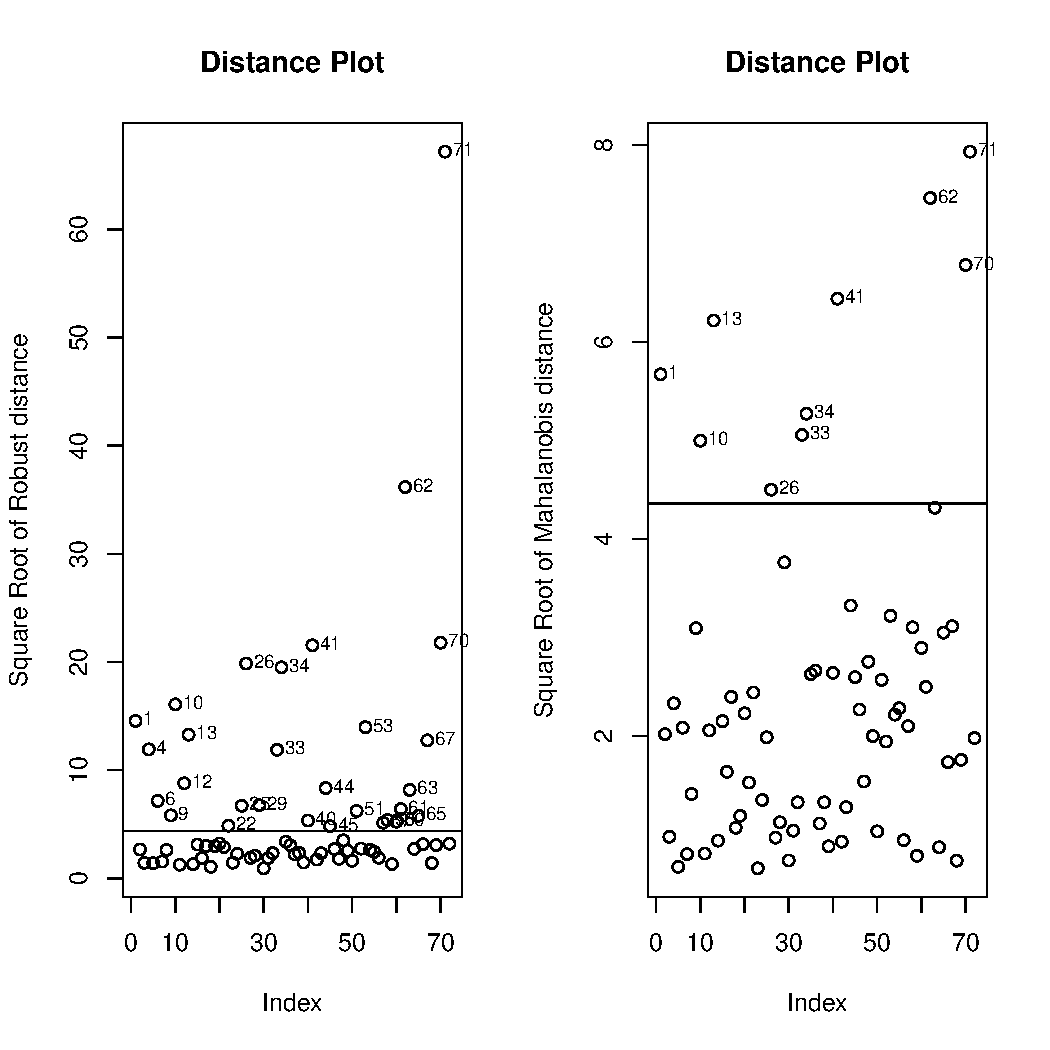
\includegraphics[width=\maxwidth]{figure/unnamed-chunk-6-1} 
\begin{kframe}\begin{alltt}
\hlnum{1}\hlopt{-}\hlkwd{length}\hlstd{(ilrdf.nafree.mcd}\hlopt{$}\hlstd{best)}\hlopt{/}\hlkwd{nrow}\hlstd{(clr.df.nafree)} \hlcom{# 43 % of outliers in this approach}
\end{alltt}
\begin{verbatim}
## [1] 0.4305556
\end{verbatim}
\end{kframe}
\end{knitrout}

Is this proportion of outliers so high a particularity of the rock ? No, one sees that with the dataframe GeoPT46, again we flag almost 43\% of observations as outliers, this is too much for practical reasons. 
cov.mcd has a default parameter alpha which is the proportion of the total sample size to take a subset of through the relationship :
\begin{align}
\alpha \times n = h
\end{align}
We can take alpha = 0.75 so this means the breakdown value of our estimator would be 25 \%.
\begin{knitrout}
\definecolor{shadecolor}{rgb}{0.969, 0.969, 0.969}\color{fgcolor}\begin{kframe}
\begin{alltt}
\hlcom{# outlier detection on the dataframe where missing values entries are replaced with column mean : }
\hlstd{ilrdf.mcd} \hlkwb{<-} \hlkwd{covMcd}\hlstd{(}\hlkwd{clr2ilr}\hlstd{(clr.df),}\hlkwc{alpha} \hlstd{=} \hlnum{.75}\hlstd{)}

\hlkwd{plot}\hlstd{(ilrdf.mcd,}\hlkwc{which} \hlstd{=} \hlkwd{c}\hlstd{(}\hlstr{"distance"}\hlstd{),}\hlkwc{classic} \hlstd{=} \hlnum{TRUE}\hlstd{)}
\end{alltt}
\end{kframe}
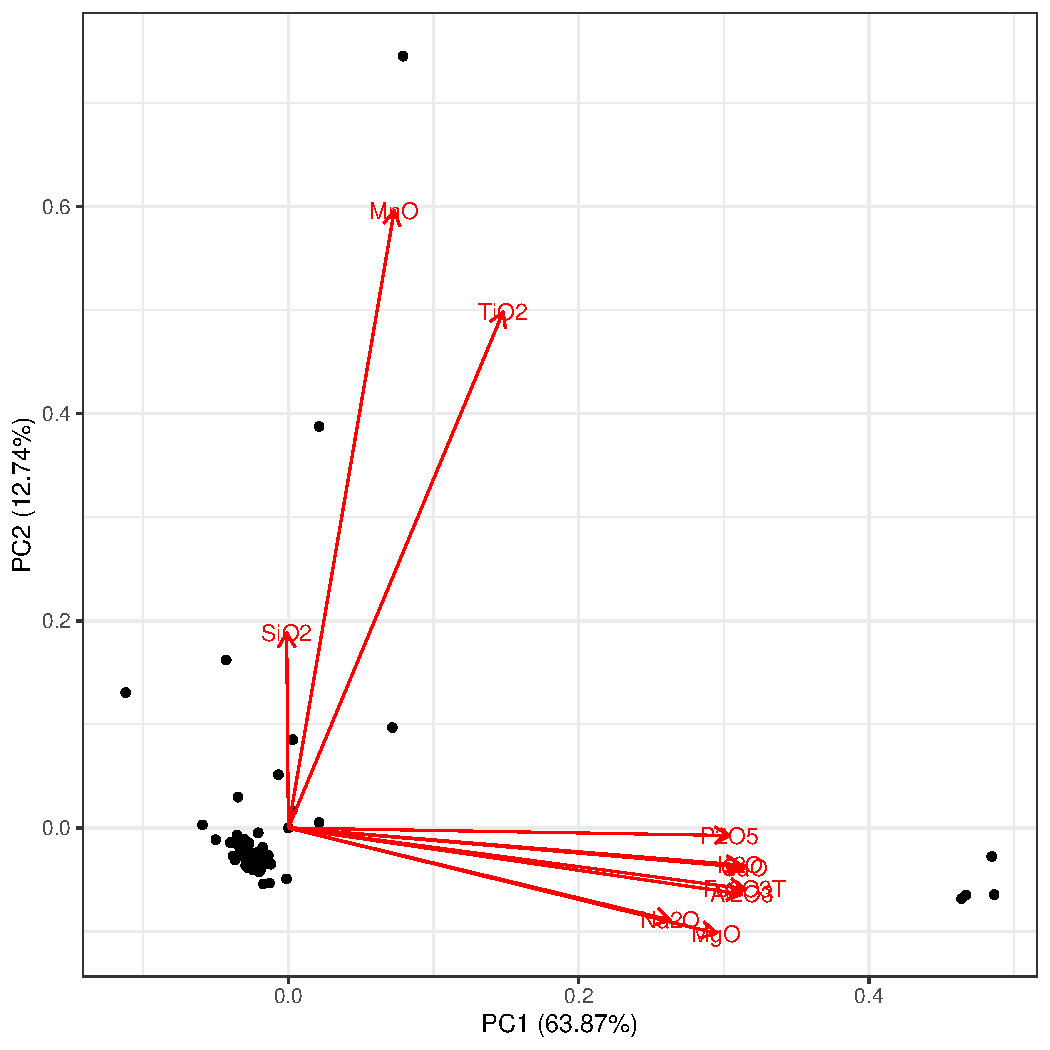
\includegraphics[width=\maxwidth]{figure/unnamed-chunk-7-1} 
\begin{kframe}\begin{alltt}
\hlnum{1}\hlopt{-}\hlkwd{length}\hlstd{(ilrdf.mcd}\hlopt{$}\hlstd{best)}\hlopt{/}\hlkwd{nrow}\hlstd{(clr.df)} \hlcom{# 22 % of outliers in this approach}
\end{alltt}
\begin{verbatim}
## [1] 0.2209302
\end{verbatim}
\begin{alltt}
\hlcom{# outlier detection on the dataframe where missing values are not taken into account}
\hlstd{ilrdf.nafree.mcd} \hlkwb{<-} \hlkwd{covMcd}\hlstd{(}\hlkwd{clr2ilr}\hlstd{(clr.df.nafree),}\hlkwc{alpha}\hlstd{=}\hlnum{.75}\hlstd{)}
\hlkwd{plot}\hlstd{(ilrdf.nafree.mcd,}\hlkwc{which} \hlstd{=} \hlkwd{c}\hlstd{(}\hlstr{"distance"}\hlstd{),}\hlkwc{classic} \hlstd{=} \hlnum{TRUE}\hlstd{)}
\end{alltt}
\end{kframe}
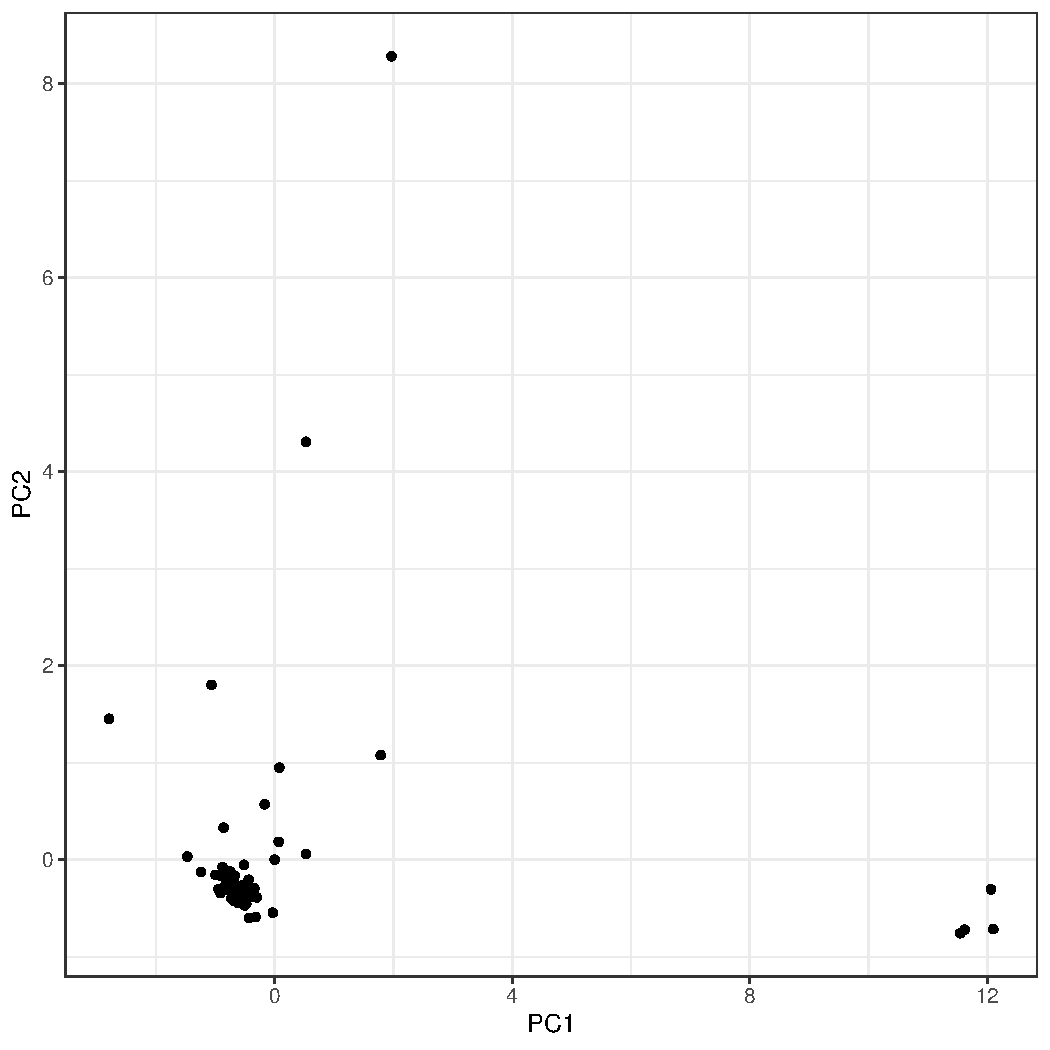
\includegraphics[width=\maxwidth]{figure/unnamed-chunk-7-2} 
\begin{kframe}\begin{alltt}
\hlnum{1}\hlopt{-}\hlkwd{length}\hlstd{(ilrdf.nafree.mcd}\hlopt{$}\hlstd{best)}\hlopt{/}\hlkwd{nrow}\hlstd{(clr.df.nafree)} \hlcom{# 22 % of outliers in this approach with robust detection method. 13 % of outliers with the non robust. }
\end{alltt}
\begin{verbatim}
## [1] 0.2222222
\end{verbatim}
\end{kframe}
\end{knitrout}





\begin{knitrout}
\definecolor{shadecolor}{rgb}{0.969, 0.969, 0.969}\color{fgcolor}\begin{kframe}
\begin{alltt}
\hlstd{ilrdf2.mcd} \hlkwb{<-} \hlkwd{covMcd}\hlstd{(}\hlkwd{clr2ilr}\hlstd{(clr.df.nafree2))}
\hlkwd{plot}\hlstd{(ilrdf2.mcd,}\hlkwc{which} \hlstd{=} \hlkwd{c}\hlstd{(}\hlstr{"distance"}\hlstd{),}\hlkwc{classic} \hlstd{=} \hlnum{TRUE}\hlstd{)}
\end{alltt}
\end{kframe}
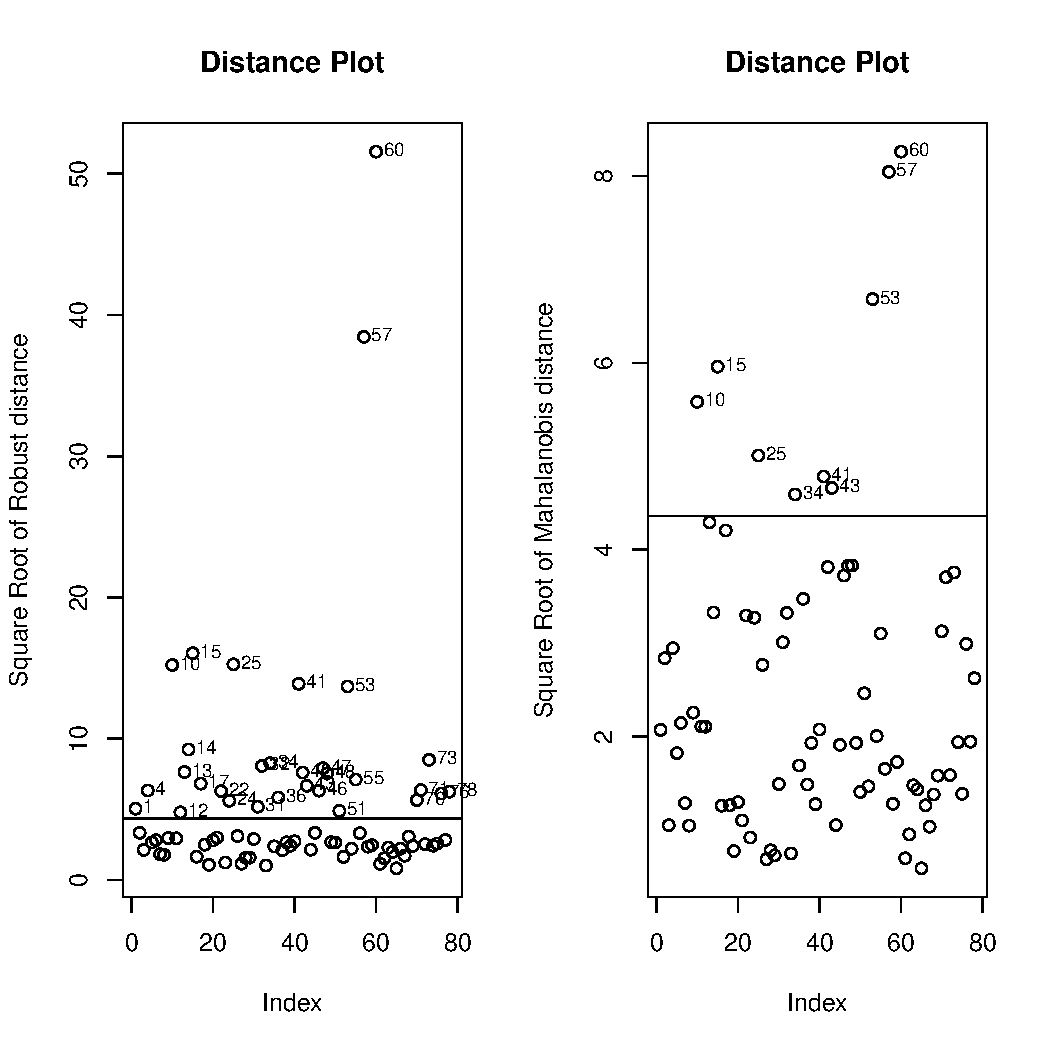
\includegraphics[width=\maxwidth]{figure/unnamed-chunk-8-1} 
\begin{kframe}\begin{alltt}
\hlnum{1}\hlopt{-}\hlkwd{length}\hlstd{(ilrdf2.mcd}\hlopt{$}\hlstd{best)}\hlopt{/}\hlkwd{nrow}\hlstd{(clr.df.nafree2)} \hlcom{# 43 % outliers in this approach, again. }
\end{alltt}
\begin{verbatim}
## [1] 0.4358974
\end{verbatim}
\end{kframe}
\end{knitrout}


Then principal component analysis is conducted.
Z denotes the mean-centered data matrix X :  
\begin{align*}
z_{ij} = x_{ij} - \mu_j
\end{align*}
Where $\mu_j$ denotes the arithmetic mean of the j-th column. Recall that here using the arithmetic mean is justified because X now lives in a subspace of $\mathbb{R}^D$ which is no longer constrained by the unit sum.

Perform Singular Value Decomposition on clr.df : 
\begin{align}
Z = UDW^T  = (UD)W^T = Z^{*}W^T,Z \in \mathbb{R}^{n\times(d-1)} U \in \mathbb{R}^{n\times p}, D \in \mathbb{R}^{p\times p}, W \in \mathbb{R}^{(d-1)\times p}
\end{align}
$Z^*$ denotes the projection of the mean-centered data matrix on a space of dimension $p$. Hopefully, $Z^*$ contains enough meaningful information about $Z$ while having a much lower number of dimensions. To evaluate how good $Z^*$ approximates $Z$, one looks at the proportion of variance explained by each of the components and more specifically, the cumulative proportion of variance explained by each of the components when these components are ranked from most to less important.



\begin{knitrout}
\definecolor{shadecolor}{rgb}{0.969, 0.969, 0.969}\color{fgcolor}\begin{kframe}
\begin{alltt}
\hlstd{pca.clr} \hlkwb{<-} \hlkwd{prcomp}\hlstd{(clr.df,}\hlkwc{scale} \hlstd{= T,}\hlkwc{rank.} \hlstd{=} \hlkwd{ncol}\hlstd{(clr.df)}\hlopt{-}\hlnum{1} \hlstd{)}
\hlkwd{summary}\hlstd{(pca.clr)}
\end{alltt}
\begin{verbatim}
## Importance of first k=9 (out of 10) components:
##                           PC1     PC2     PC3    PC4     PC5     PC6     PC7
## Standard deviation     2.6562 0.97703 0.91318 0.7470 0.56855 0.34083 0.25171
## Proportion of Variance 0.7055 0.09546 0.08339 0.0558 0.03233 0.01162 0.00634
## Cumulative Proportion  0.7055 0.80098 0.88437 0.9402 0.97249 0.98411 0.99045
##                            PC8     PC9
## Standard deviation     0.24623 0.18687
## Proportion of Variance 0.00606 0.00349
## Cumulative Proportion  0.99651 1.00000
\end{verbatim}
\begin{alltt}
\hlcom{# repeat for nafree df}
\hlstd{pca.clr.nafree} \hlkwb{<-} \hlkwd{prcomp}\hlstd{(clr.df.nafree,}\hlkwc{scale} \hlstd{= T,}\hlkwc{rank.} \hlstd{=} \hlkwd{ncol}\hlstd{(clr.df)}\hlopt{-}\hlnum{1} \hlstd{)}
\hlkwd{summary}\hlstd{(pca.clr.nafree)}
\end{alltt}
\begin{verbatim}
## Importance of first k=9 (out of 10) components:
##                           PC1    PC2    PC3     PC4     PC5     PC6     PC7
## Standard deviation     2.2003 1.4357 1.0267 0.77238 0.73015 0.66663 0.51892
## Proportion of Variance 0.4841 0.2061 0.1054 0.05966 0.05331 0.04444 0.02693
## Cumulative Proportion  0.4841 0.6902 0.7957 0.85531 0.90863 0.95307 0.97999
##                            PC8     PC9
## Standard deviation     0.37047 0.25063
## Proportion of Variance 0.01372 0.00628
## Cumulative Proportion  0.99372 1.00000
\end{verbatim}
\end{kframe}
\end{knitrout}
The importance of a component, in terms of proportion of variance explained, is directly related to the D matrix whose eigenvalues squared are directly related to the proportion of variance explained through the relationship : 
\begin{align} \label{variancepca}
\lambda_i = d_i^2/(n-1)
\end{align}
Where $d_i$ denotes the i-th diagonal element in the square matrix D of the singular values and n is the number of principal components which is equal to the dimensionality of the original data matrix X.

Now, one looks at the rank-two approximation of Z (as the biplot does) :
\begin{knitrout}
\definecolor{shadecolor}{rgb}{0.969, 0.969, 0.969}\color{fgcolor}\begin{kframe}
\begin{alltt}
\hlcom{# autoplot}
\hlkwd{autoplot}\hlstd{(pca.clr,}\hlkwc{loadings}\hlstd{=T,}\hlkwc{loadings.label}\hlstd{=T)}\hlopt{+}\hlkwd{theme_bw}\hlstd{()}
\end{alltt}
\end{kframe}
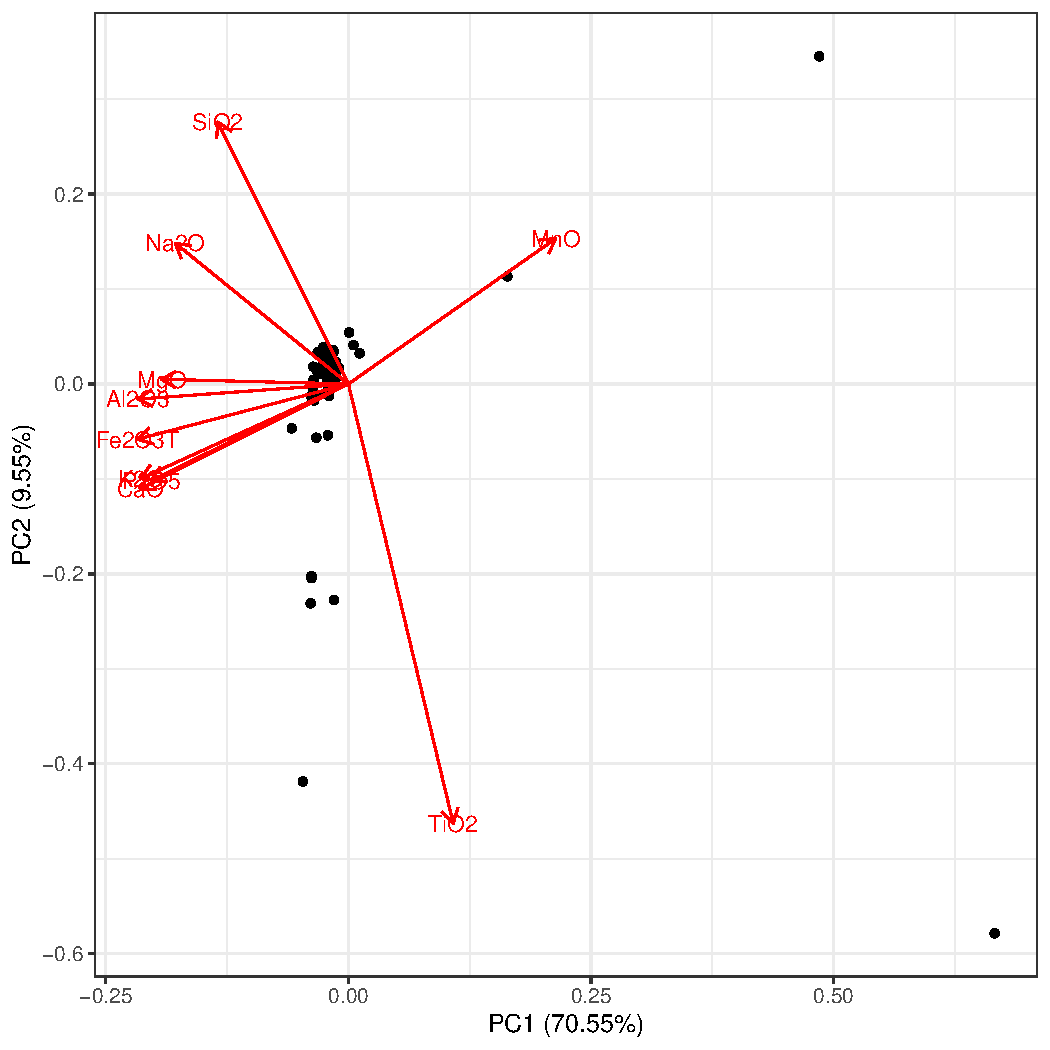
\includegraphics[width=\maxwidth]{figure/unnamed-chunk-10-1} 
\begin{kframe}\begin{alltt}
\hlkwd{autoplot}\hlstd{(pca.clr.nafree,}\hlkwc{loadings}\hlstd{=T,}\hlkwc{loadings.label}\hlstd{=T)}\hlopt{+}\hlkwd{theme_bw}\hlstd{()}
\end{alltt}
\end{kframe}
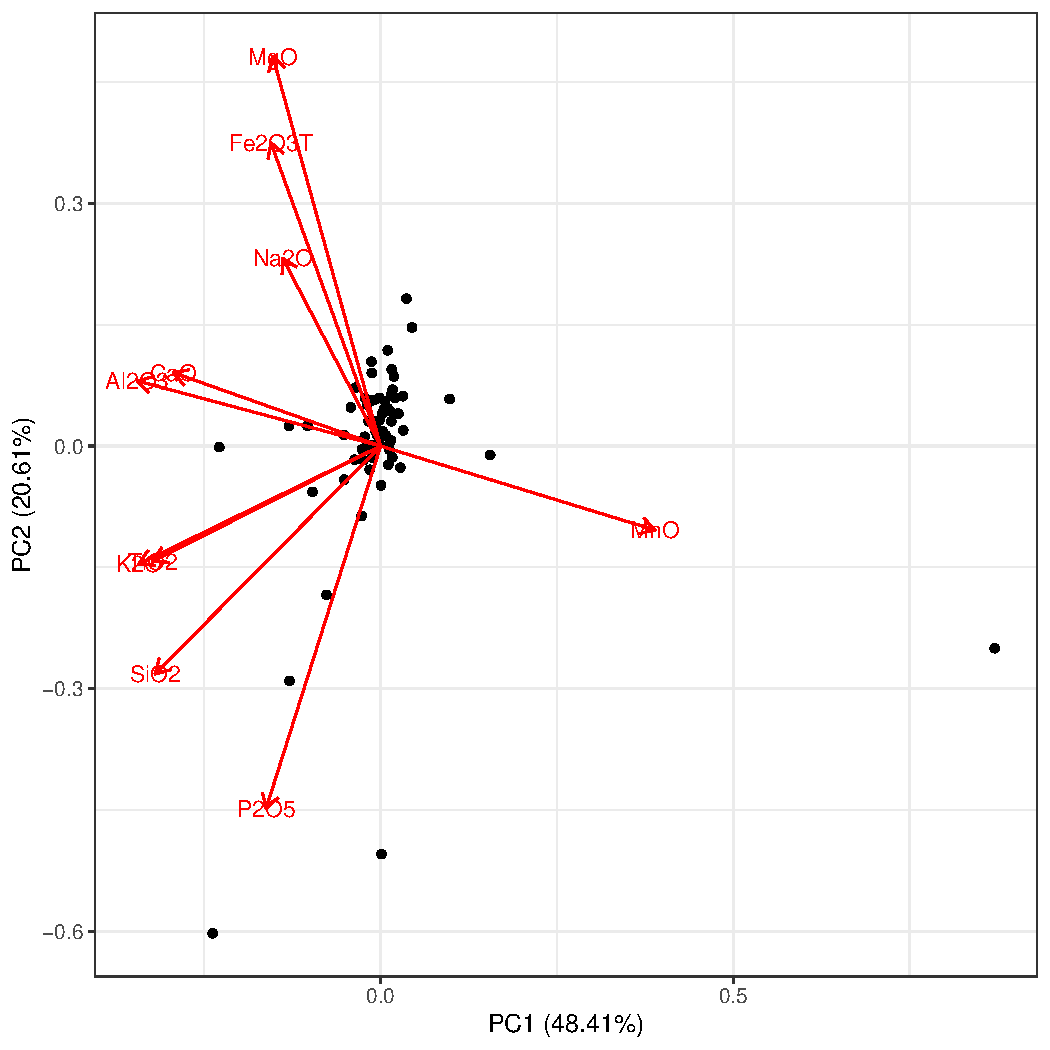
\includegraphics[width=\maxwidth]{figure/unnamed-chunk-10-2} 
\begin{kframe}\begin{alltt}
\hlcom{# manually extracting the rank 2 approximation of Z}
\hlstd{Z.approx} \hlkwb{<-} \hlkwd{data.frame}\hlstd{(pca.clr}\hlopt{$}\hlstd{x[,}\hlkwd{c}\hlstd{(}\hlnum{1}\hlstd{,}\hlnum{2}\hlstd{)])}
\hlkwd{colnames}\hlstd{(Z.approx)} \hlkwb{=} \hlkwd{c}\hlstd{(}\hlstr{"PC1"}\hlstd{,}\hlstr{"PC2"}\hlstd{)}
\hlkwd{ggplot}\hlstd{(}\hlkwd{aes}\hlstd{(}\hlkwc{x}\hlstd{=PC1,}\hlkwc{y}\hlstd{=PC2),}\hlkwc{data}\hlstd{=Z.approx)}\hlopt{+}\hlkwd{theme_bw}\hlstd{()}\hlopt{+}\hlkwd{geom_point}\hlstd{()}
\end{alltt}
\end{kframe}
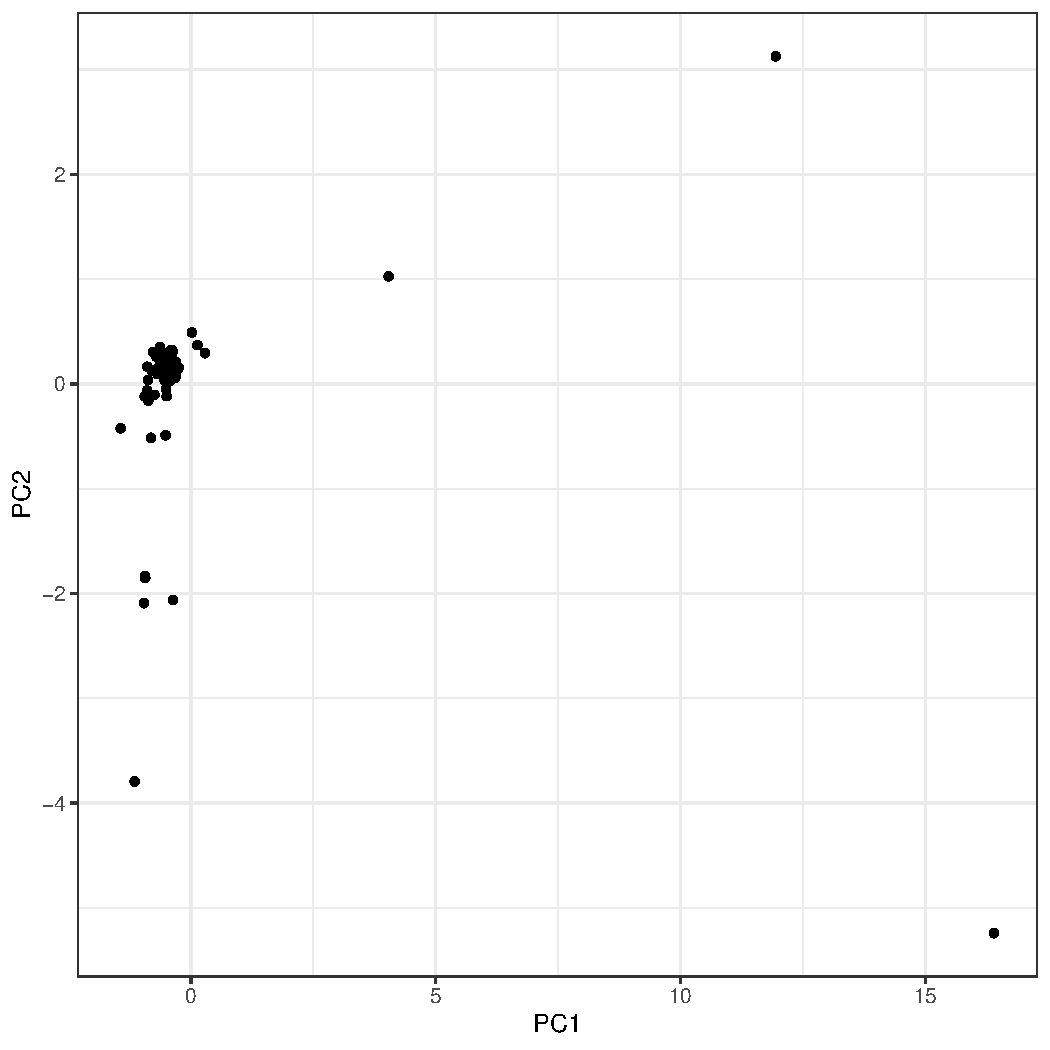
\includegraphics[width=\maxwidth]{figure/unnamed-chunk-10-3} 
\end{knitrout}
Flagging the outliers, remarkable discrepancy between robust method (MCD estimator of the location, MCD is affine equivariant and has a high breakdown value) vs classical method (sample covariance matrix). 
\begin{knitrout}
\definecolor{shadecolor}{rgb}{0.969, 0.969, 0.969}\color{fgcolor}\begin{kframe}
\begin{alltt}
\hlstd{Z2.mcd} \hlkwb{<-} \hlkwd{covMcd}\hlstd{(Z.approx,}\hlkwc{alpha} \hlstd{=} \hlnum{0.75}\hlstd{)}
\hlkwd{tolEllipsePlot}\hlstd{(Z.approx,}\hlkwc{classic} \hlstd{= T,}\hlkwc{m.cov} \hlstd{= Z2.mcd)}
\end{alltt}
\end{kframe}
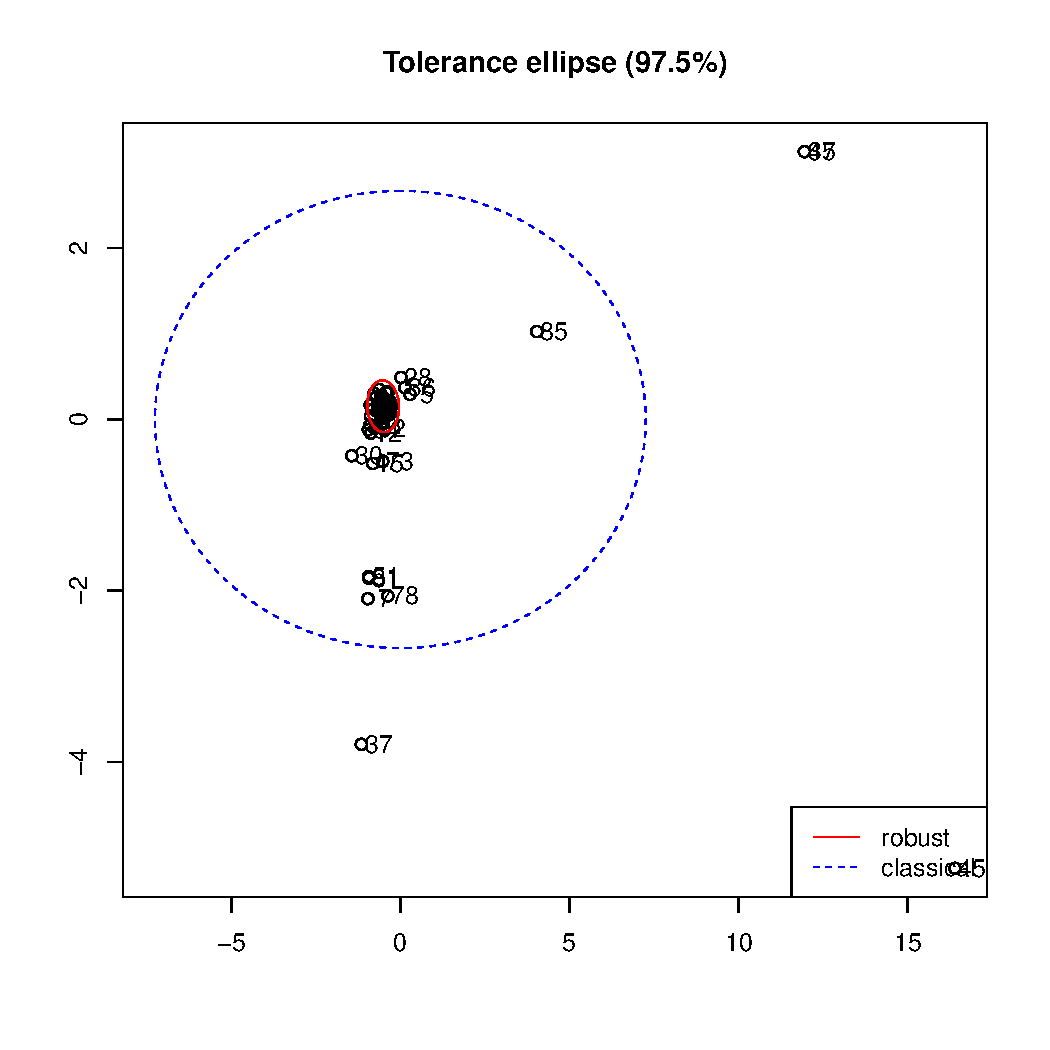
\includegraphics[width=\maxwidth]{figure/unnamed-chunk-11-1} 
\begin{kframe}\begin{alltt}
\hlkwd{plot}\hlstd{(Z2.mcd,}\hlkwc{which} \hlstd{=} \hlkwd{c}\hlstd{(}\hlstr{"distance"}\hlstd{),}\hlkwc{classic} \hlstd{=} \hlnum{TRUE}\hlstd{)}
\end{alltt}
\end{kframe}
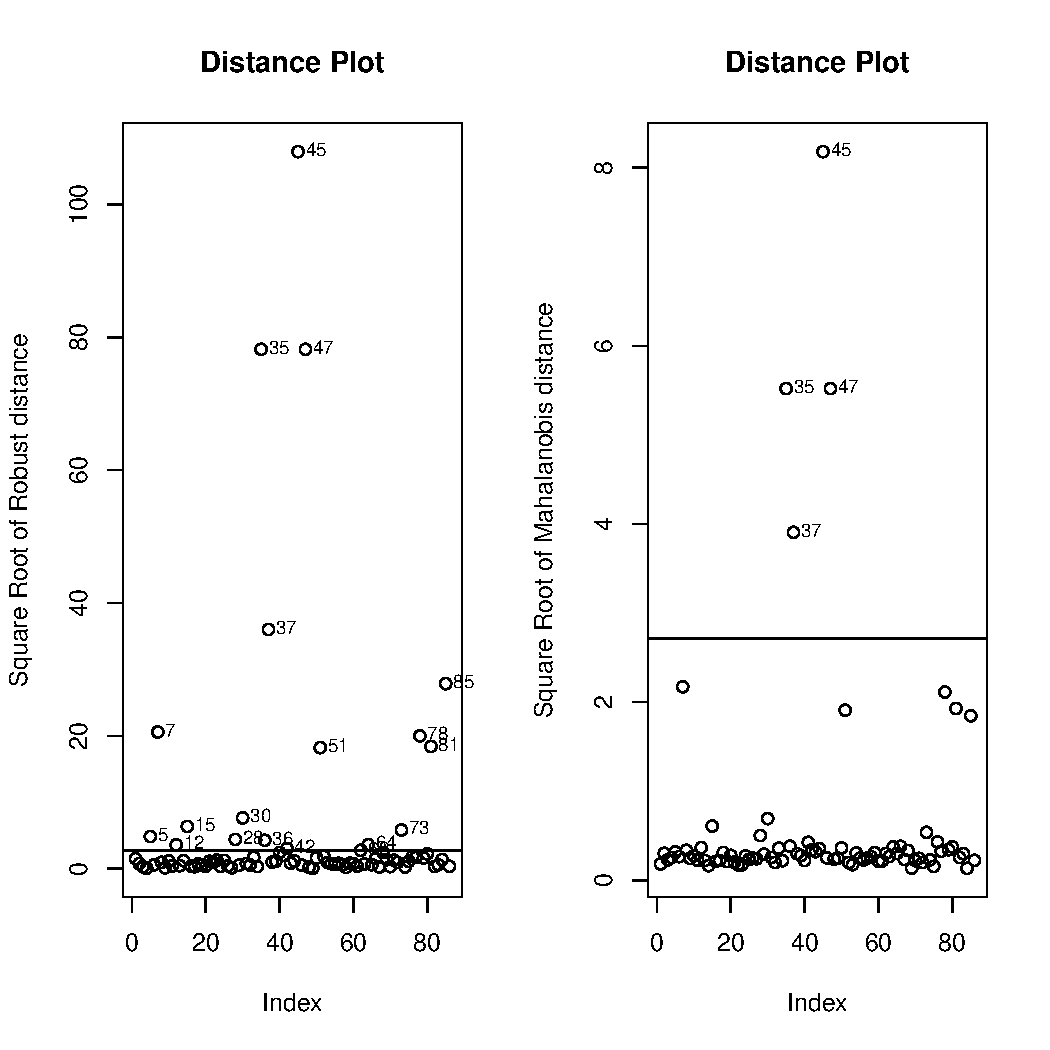
\includegraphics[width=\maxwidth]{figure/unnamed-chunk-11-2} 
\begin{kframe}\begin{alltt}
\hlstd{Z2.outfree} \hlkwb{<-} \hlstd{Z.approx[Z2.mcd}\hlopt{$}\hlstd{best,]}
\hlkwd{nrow}\hlstd{(Z2.outfree)}\hlopt{/}\hlkwd{nrow}\hlstd{(Z.approx)}
\end{alltt}
\begin{verbatim}
## [1] 0.755814
\end{verbatim}
\end{kframe}
\end{knitrout}
This approach has a pitfall. The estimation of the PC is itself not robust. Robcompositions package provides a robust PCA estimation method :
\begin{quote}
The compositional data set is expressed in isometric logratio coordinates. Afterwards, robust principal component analysis is performed. Resulting loadings and scores are back-transformed to the clr space where the compositional biplot can be shown. CITE ROBCOMP R package
\end{quote}
\begin{knitrout}
\definecolor{shadecolor}{rgb}{0.969, 0.969, 0.969}\color{fgcolor}\begin{kframe}
\begin{alltt}
\hlstd{rob.pca.clr} \hlkwb{<-} \hlkwd{pcaCoDa}\hlstd{(df.majors)}
\hlkwd{summary}\hlstd{(rob.pca.clr)}
\end{alltt}
\begin{verbatim}
## Importance of components:
##                           Comp.1     Comp.2     Comp.3     Comp.4    Comp.5
## Standard deviation     0.0730207 0.03302854 0.03242246 0.02468697 0.0205167
## Proportion of Variance 0.5873237 0.12016122 0.11579171 0.06713070 0.0463661
## Cumulative Proportion  0.5873237 0.70748494 0.82327665 0.89040735 0.9367734
##                            Comp.6     Comp.7      Comp.8      Comp.9
## Standard deviation     0.01848889 0.01108852 0.009229454 0.004901582
## Proportion of Variance 0.03765368 0.01354355 0.009382911 0.002646416
## Cumulative Proportion  0.97442713 0.98797067 0.997353584 1.000000000
\end{verbatim}
\end{kframe}
\end{knitrout}
One sees that the first two PC's found by using the robust method explains (89 \%) whereas in the classical method, the first two PC's explained only 76 \%. The outlier detection is repeated in the first 2 robust PC's subspace.
\begin{knitrout}
\definecolor{shadecolor}{rgb}{0.969, 0.969, 0.969}\color{fgcolor}\begin{kframe}
\begin{alltt}
\hlstd{Z.approx.rob} \hlkwb{<-} \hlkwd{data.frame}\hlstd{(rob.pca.clr}\hlopt{$}\hlstd{scores[,}\hlkwd{c}\hlstd{(}\hlnum{1}\hlstd{,}\hlnum{2}\hlstd{)])}
\hlkwd{colnames}\hlstd{(Z.approx.rob)} \hlkwb{=} \hlkwd{c}\hlstd{(}\hlstr{"PC1"}\hlstd{,}\hlstr{"PC2"}\hlstd{)}
\hlkwd{ggplot}\hlstd{(}\hlkwd{aes}\hlstd{(}\hlkwc{x}\hlstd{=PC1,}\hlkwc{y}\hlstd{=PC2),}\hlkwc{data}\hlstd{=Z.approx.rob)}\hlopt{+}\hlkwd{theme_bw}\hlstd{()}\hlopt{+}\hlkwd{geom_point}\hlstd{()}
\end{alltt}
\end{kframe}
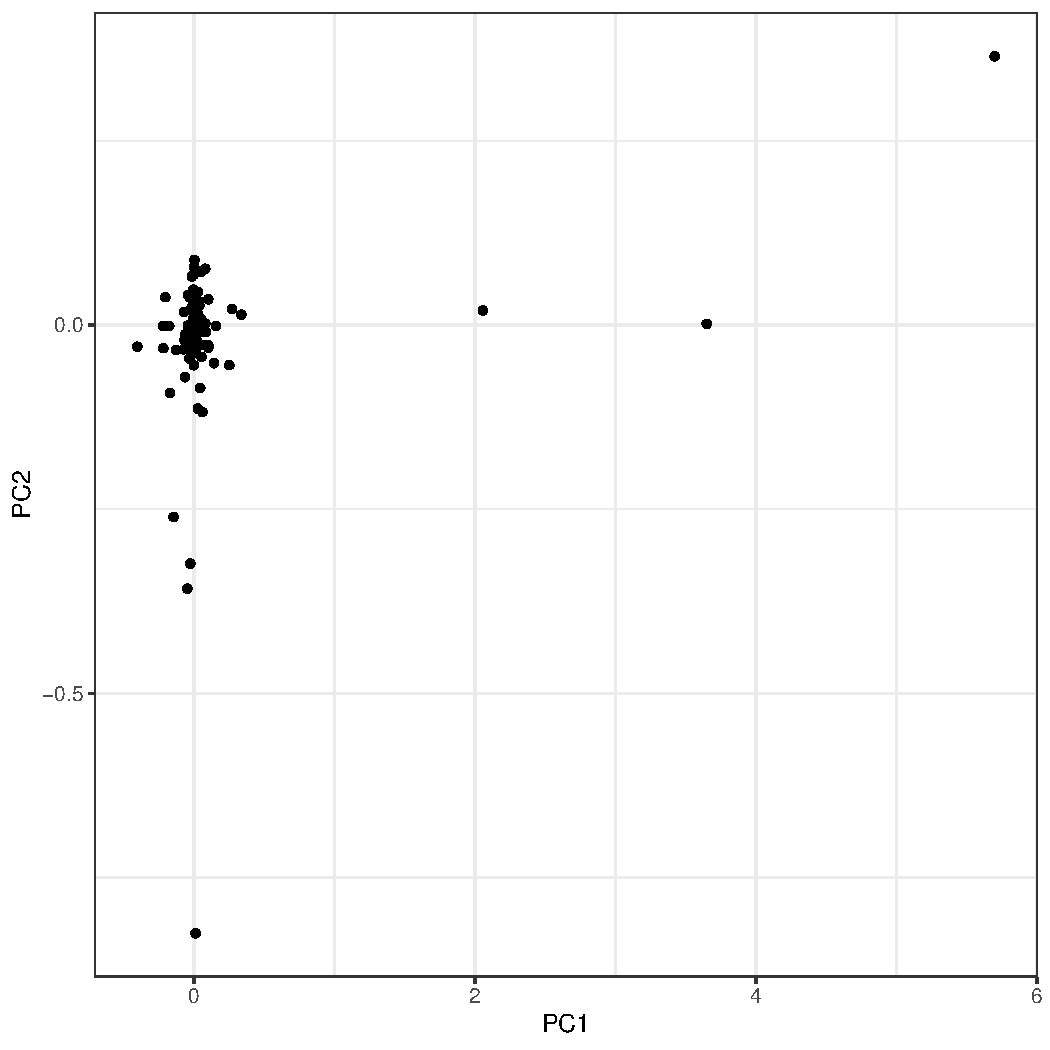
\includegraphics[width=\maxwidth]{figure/unnamed-chunk-13-1} 
\end{knitrout}
At first glance, there seem to be less outliers in the robust first two PC's space. This is checked by using diagnostic plots : 
\begin{knitrout}
\definecolor{shadecolor}{rgb}{0.969, 0.969, 0.969}\color{fgcolor}\begin{kframe}
\begin{alltt}
\hlstd{Z2.rob.mcd} \hlkwb{<-} \hlkwd{covMcd}\hlstd{(Z.approx.rob,)}
\hlkwd{tolEllipsePlot}\hlstd{(Z.approx.rob,}\hlkwc{classic} \hlstd{= T)}
\end{alltt}
\end{kframe}
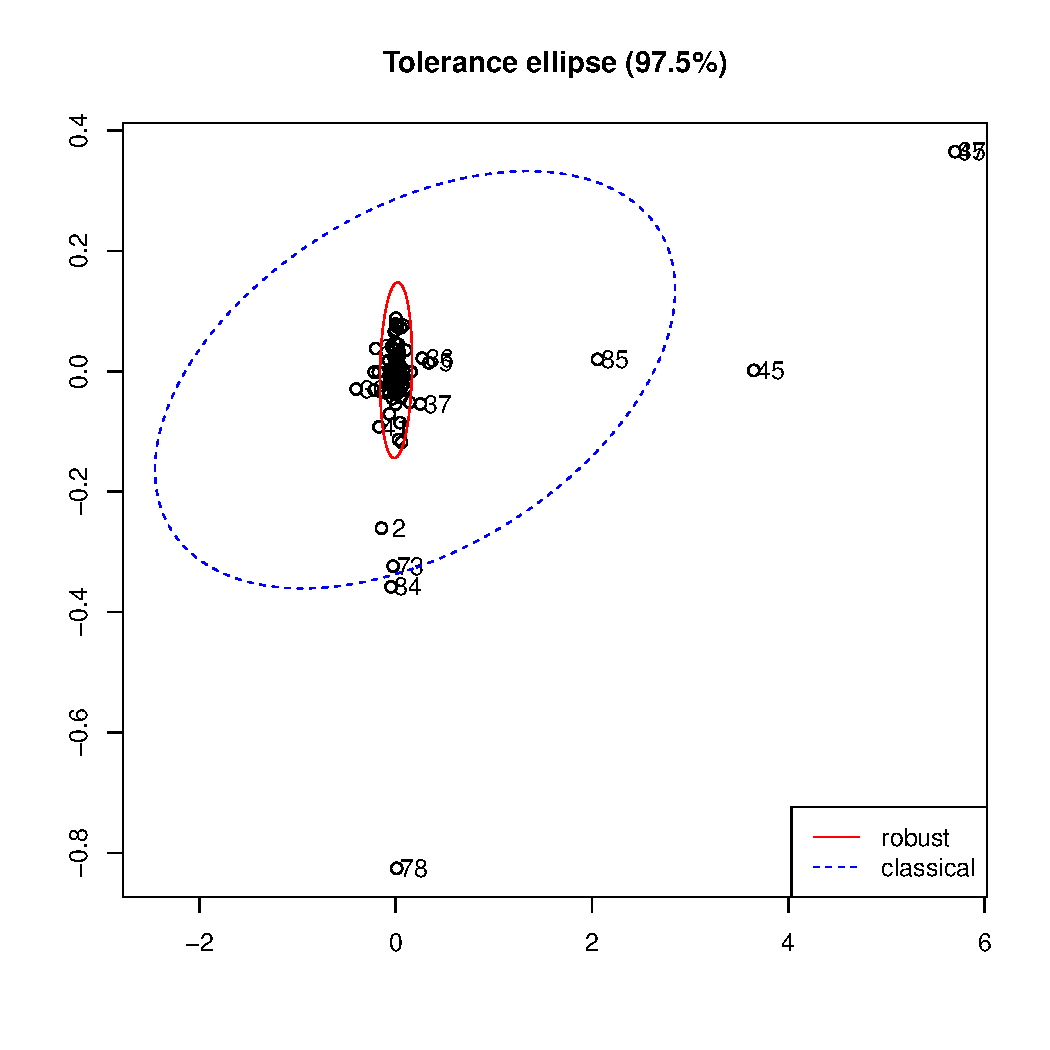
\includegraphics[width=\maxwidth]{figure/unnamed-chunk-14-1} 
\begin{kframe}\begin{alltt}
\hlkwd{plot}\hlstd{(Z2.rob.mcd,}\hlkwc{which} \hlstd{=} \hlkwd{c}\hlstd{(}\hlstr{"distance"}\hlstd{),}\hlkwc{classic} \hlstd{=} \hlnum{TRUE}\hlstd{)}
\end{alltt}
\end{kframe}
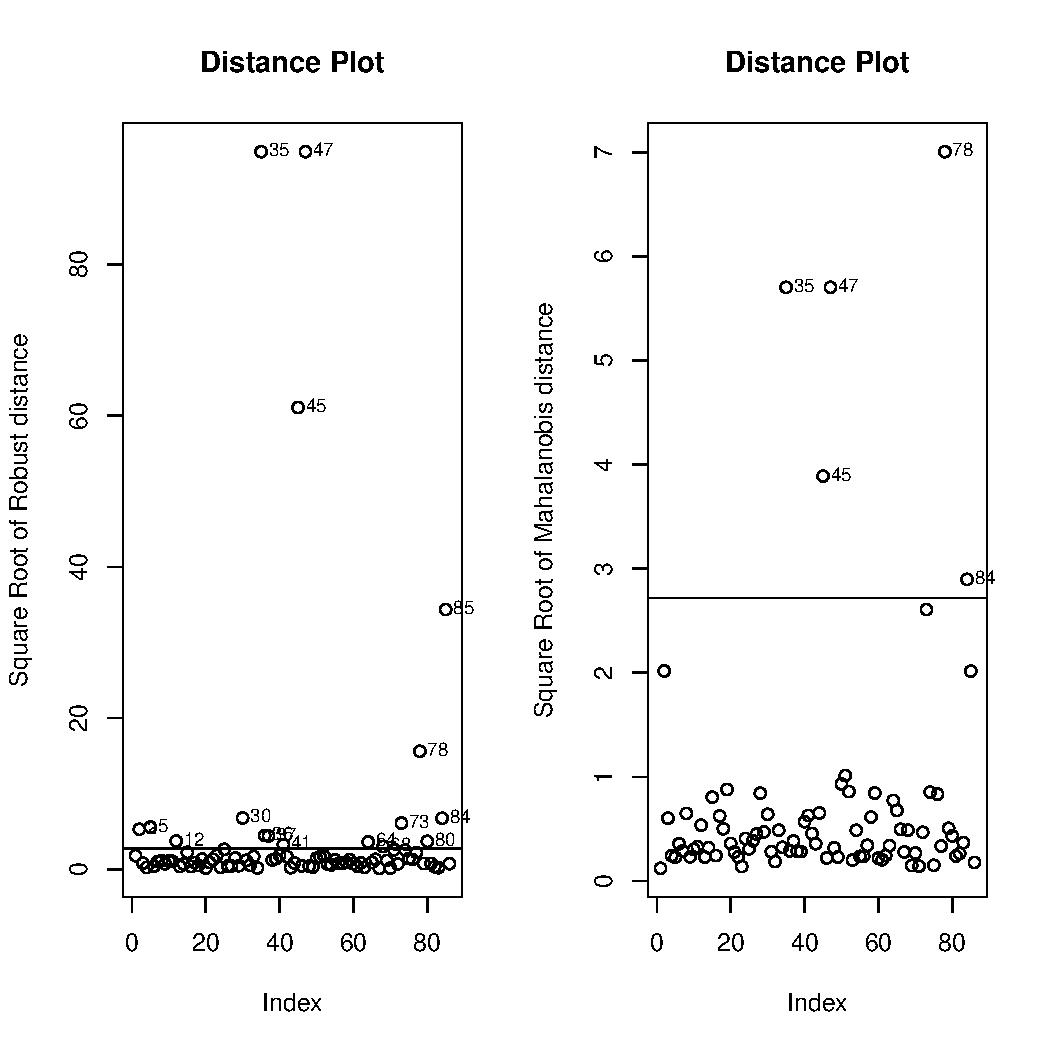
\includegraphics[width=\maxwidth]{figure/unnamed-chunk-14-2} 
\begin{kframe}\begin{alltt}
\hlstd{Z2.rob.outfree} \hlkwb{<-} \hlstd{Z.approx.rob[Z2.rob.mcd}\hlopt{$}\hlstd{best,]}
\hlkwd{ggplot}\hlstd{(}\hlkwd{aes}\hlstd{(}\hlkwc{x}\hlstd{=PC1,}\hlkwc{y}\hlstd{=PC2),}\hlkwc{data}\hlstd{=Z2.rob.outfree)}\hlopt{+}\hlkwd{theme_bw}\hlstd{()}\hlopt{+}\hlkwd{geom_point}\hlstd{()}\hlopt{+}\hlkwd{stat_ellipse}\hlstd{()}
\end{alltt}
\end{kframe}
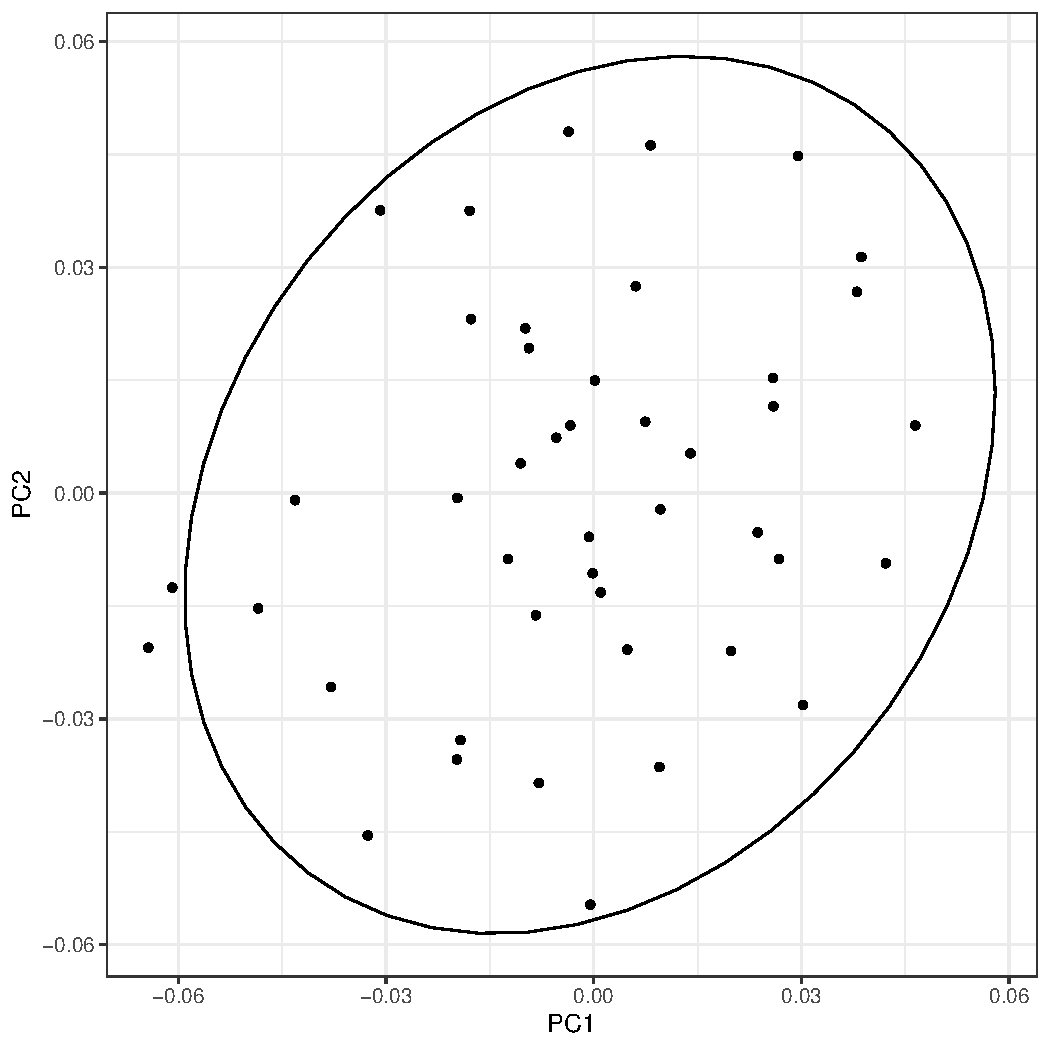
\includegraphics[width=\maxwidth]{figure/unnamed-chunk-14-3} 
\end{knitrout}
There seems to be no association between PC1 and PC2, which makes much more sense. Eventually, an estimation for rock 1 composition is
\begin{knitrout}
\definecolor{shadecolor}{rgb}{0.969, 0.969, 0.969}\color{fgcolor}\begin{kframe}
\begin{alltt}
\hlstd{df.majors.out.free} \hlkwb{<-} \hlstd{df.majors[Z2.rob.mcd}\hlopt{$}\hlstd{best,]}
\hlstd{df.majors.out.free.clr} \hlkwb{<-} \hlkwd{data.frame}\hlstd{(}\hlkwd{clr}\hlstd{(df.majors.out.free))}
\hlstd{clr.mean} \hlkwb{<-} \hlkwd{colMeans}\hlstd{(df.majors.out.free.clr)}
\hlstd{clr.cov} \hlkwb{<-} \hlkwd{Cov}\hlstd{(df.majors.out.free.clr)}

\hlstd{mean.estimate} \hlkwb{<-} \hlkwd{as.vector}\hlstd{(}\hlkwd{clrInv}\hlstd{(clr.mean))}
\hlstd{cov.estimate} \hlkwb{<-} \hlkwd{clrInv}\hlstd{(}\hlkwd{as.matrix}\hlstd{(clr.cov}\hlopt{$}\hlstd{cov))}
\hlstd{cov.estimate}
\end{alltt}
\begin{verbatim}
##        SiO2         TiO2         Al2O3        Fe2O3T       MnO        
## SiO2   "0.10289487" "0.09962841" "0.09987669" "0.09979176" "0.0996833"
## TiO2   "0.09963294" "0.10007568" "0.10001475" "0.10002610" "0.1000330"
## Al2O3  "0.09988130" "0.10001482" "0.10002404" "0.10001191" "0.1000105"
## Fe2O3T "0.09979635" "0.10002615" "0.10001190" "0.10005504" "0.1000140"
## MnO    "0.09968785" "0.10003302" "0.10001042" "0.10001398" "0.1000981"
## MgO    "0.09971372" "0.10001797" "0.10000860" "0.10001880" "0.1000277"
## CaO    "0.09959408" "0.10005293" "0.10000200" "0.10002234" "0.1000343"
## Na2O   "0.09966646" "0.10004172" "0.10001381" "0.09999442" "0.1000451"
## K2O    "0.09967389" "0.10004639" "0.10001272" "0.10003256" "0.1000178"
## P2O5   "0.09949945" "0.10005849" "0.10001994" "0.10002814" "0.1000317"
##        MgO          CaO          Na2O         K2O          P2O5        
## SiO2   "0.09970915" "0.09958957" "0.09966191" "0.09966934" "0.09949499"
## TiO2   "0.10001794" "0.10005295" "0.10004171" "0.10004637" "0.10005855"
## Al2O3  "0.10000864" "0.10000209" "0.10001387" "0.10001277" "0.10002008"
## Fe2O3T "0.10001883" "0.10002242" "0.09999446" "0.10003259" "0.10002826"
## MnO    "0.10002772" "0.10003430" "0.10004514" "0.10001776" "0.10003176"
## MgO    "0.10008386" "0.10003285" "0.10002368" "0.10002052" "0.10005227"
## CaO    "0.10003280" "0.10009855" "0.10004622" "0.10004775" "0.10006905"
## Na2O   "0.10002366" "0.10004625" "0.10009211" "0.10002929" "0.10004714"
## K2O    "0.10002050" "0.10004779" "0.10002930" "0.10005981" "0.10005929"
## P2O5   "0.10005218" "0.10006900" "0.10004706" "0.10005921" "0.10013487"
## attr(,"class")
## [1] "acomp"
\end{verbatim}
\end{kframe}
\end{knitrout}
How does it compare with the naive estimates of GeoPT ? 
\begin{knitrout}
\definecolor{shadecolor}{rgb}{0.969, 0.969, 0.969}\color{fgcolor}\begin{kframe}
\begin{alltt}
\hlstd{mean.naive} \hlkwb{<-} \hlkwd{colMeans}\hlstd{(}\hlkwd{clo}\hlstd{(df.majors))}
\hlstd{od} \hlkwb{<-} \hlkwd{outCoDa}\hlstd{(df.majors,} \hlkwc{quantile} \hlstd{=} \hlnum{0.975}\hlstd{,} \hlkwc{method} \hlstd{=} \hlstr{"robust"}\hlstd{,} \hlkwc{alpha} \hlstd{=} \hlnum{0.9}\hlstd{,} \hlkwc{coda} \hlstd{=} \hlnum{TRUE}\hlstd{)}
\hlstd{df.major.wo.outliers} \hlkwb{<-} \hlstd{df.majors[od}\hlopt{$}\hlstd{outlierIndex,]}
\hlstd{mean.naive.wo.outlier} \hlkwb{<-} \hlkwd{colMeans}\hlstd{(}\hlkwd{clo}\hlstd{(df.major.wo.outliers))}
\end{alltt}
\end{kframe}
\end{knitrout}
Not much difference for SiO2 \emph{but} TiO2 concentration is twice as high in the naive way, 5 times higher in the naive way when removing outliers. MnO concentration is 10 times higher in the naive way. 
\begin{knitrout}
\definecolor{shadecolor}{rgb}{0.969, 0.969, 0.969}\color{fgcolor}\begin{kframe}
\begin{alltt}
\hlstd{df} \hlkwb{<-} \hlkwd{data.frame}\hlstd{(mean.estimate,mean.naive,mean.naive.wo.outlier)}
\hlstd{df}
\end{alltt}
\begin{verbatim}
##        mean.estimate  mean.naive mean.naive.wo.outlier
## SiO2     0.572280369 0.562480850           0.509635270
## TiO2     0.011132233 0.016099834           0.030527015
## Al2O3    0.201225261 0.197964339           0.200463923
## Fe2O3T   0.049229936 0.048373292           0.048931757
## MnO      0.001432903 0.013702982           0.047356073
## MgO      0.011614807 0.011273968           0.011162882
## CaO      0.038608273 0.038366921           0.040530951
## Na2O     0.069131939 0.066717132           0.064349912
## K2O      0.039169507 0.038844793           0.040388171
## P2O5     0.006174773 0.006175889           0.006654047
\end{verbatim}
\begin{alltt}
\hlstd{df}\hlopt{$}\hlstd{element} \hlkwb{<-} \hlkwd{row.names}\hlstd{(df)}
\hlstd{df.plot} \hlkwb{<-} \hlstd{df} \hlopt \hlkwd{pivot_longer}\hlstd{(}\hlkwc{cols}\hlstd{=}\hlkwd{starts_with}\hlstd{(}\hlstr{"mean"}\hlstd{))}
\hlstd{df.plot}
\end{alltt}
\begin{verbatim}
## # A tibble: 30 x 3
##    element name                   value
##    <chr>   <chr>                  <dbl>
##  1 SiO2    mean.estimate         0.572 
##  2 SiO2    mean.naive            0.562 
##  3 SiO2    mean.naive.wo.outlier 0.510 
##  4 TiO2    mean.estimate         0.0111
##  5 TiO2    mean.naive            0.0161
##  6 TiO2    mean.naive.wo.outlier 0.0305
##  7 Al2O3   mean.estimate         0.201 
##  8 Al2O3   mean.naive            0.198 
##  9 Al2O3   mean.naive.wo.outlier 0.200 
## 10 Fe2O3T  mean.estimate         0.0492
## # ... with 20 more rows
\end{verbatim}
\begin{alltt}
\hlstd{df.plot}\hlopt{$}\hlstd{group} \hlkwb{<-} \hlkwd{ifelse}\hlstd{(df.plot}\hlopt{$}\hlstd{element} \hlopt \hlkwd{c}\hlstd{(}\hlstr{"SiO2"}\hlstd{,}\hlstr{"Al2O3"}\hlstd{),}\hlkwc{yes} \hlstd{=} \hlstr{"large"}\hlstd{,}\hlstr{"small"}\hlstd{)}
\hlkwd{ggplot}\hlstd{(}\hlkwd{aes}\hlstd{(}\hlkwc{x}\hlstd{=element,}\hlkwc{y}\hlstd{=value),}\hlkwc{data} \hlstd{= df.plot)}\hlopt{+}\hlkwd{geom_col}\hlstd{(}\hlkwd{aes}\hlstd{(}\hlkwc{fill}\hlstd{=name),}\hlkwc{position} \hlstd{=} \hlstr{"dodge"}\hlstd{)}\hlopt{+}\hlkwd{theme_bw}\hlstd{()}\hlopt{+}\hlkwd{facet_grid}\hlstd{(group}\hlopt{~}\hlstd{.,}\hlkwc{scales} \hlstd{=} \hlstr{"free"}\hlstd{)}\hlopt{+}\hlkwd{scale_color_viridis_d}\hlstd{()}
\end{alltt}
\end{kframe}
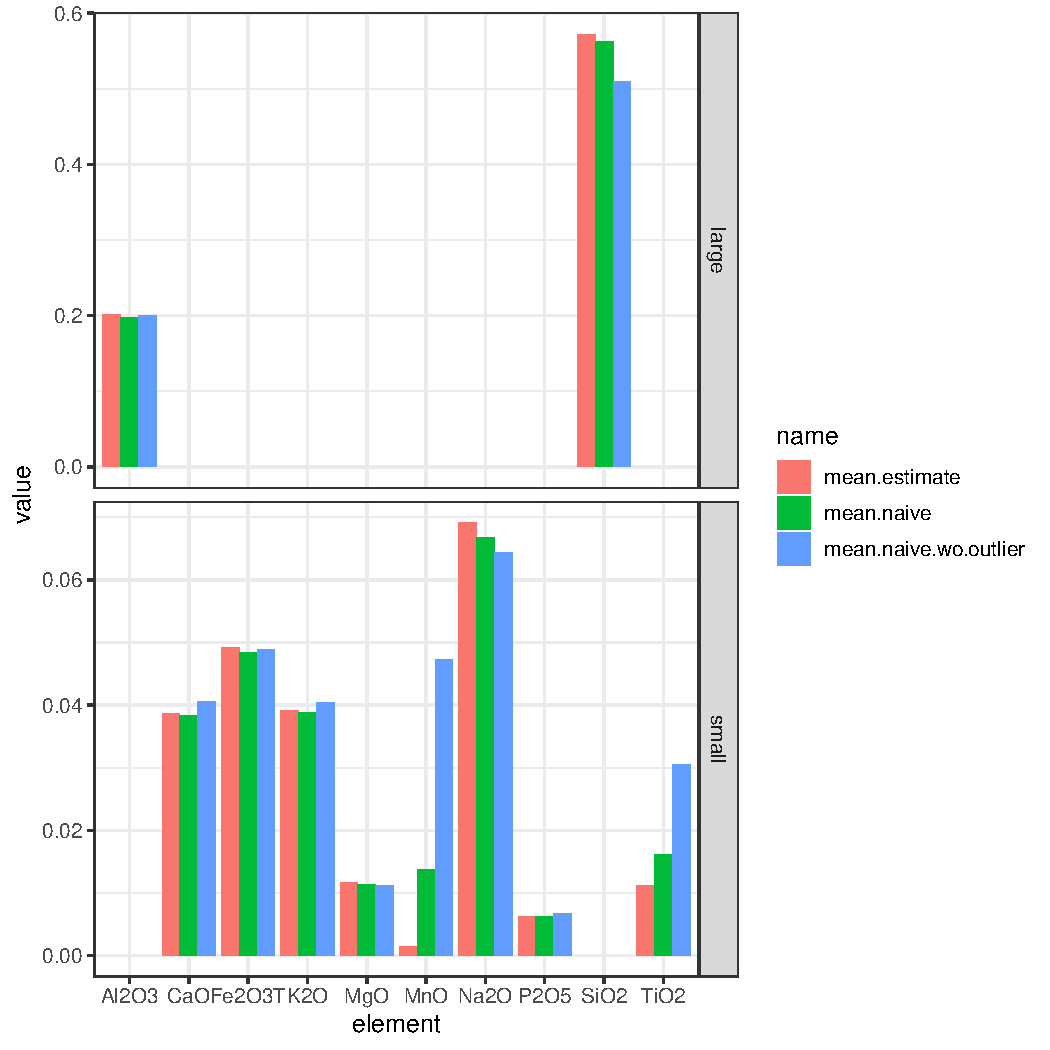
\includegraphics[width=\maxwidth]{figure/unnamed-chunk-17-1} 
\end{knitrout}
Preliminary conclusion : naive without outlier downplay the concentration of elements present in large quantities and blow the concentration of elements present in small quantities.




\end{document}
